\documentclass[a4paper,11pt]{article}
\usepackage[czech]{babel}
\usepackage[a4paper, total={7in, 10in}]{geometry} % Border sizes
\usepackage[T1]{fontenc} % LaTeX default font encoding 
\usepackage{multirow} % LaTeX multirow package for table
\usepackage{titlesec} % LaTeX titlesec package for section title changes
\usepackage{sectsty} % For section styles
\usepackage{multicol} % For multi-column tables
\usepackage{graphicx} % For images
\usepackage{gensymb} % For degree /degree
\usepackage{charter} % use the charter font
\usepackage{enumitem} % Enumerated item list
\usepackage{tabularx}

\sectionfont{\centering} % Center section title
\def\svgwidth{\columnwidth} % Set width of svg images to column width
\newcommand{\textoverline}[1]{$\overline{\mbox{#1}}$} % For overline on text

\begin{document}
\pagenumbering{gobble} % Remove page numbers

\section*{Maturitní otázky TVY+POS}
\begin{center}
    \Large Karel Bašta - V4D
\end{center}
\begin{enumerate}
    \item ISO-OSI (význam a popis), TCP/IP (význam, popis, vztah k ISO/OSI)
    \item Polovodičové paměti (základní rozdělení, realizace buňky statické a dynamické paměti, R/W cyklus vybrané buňky)
    \item VLAN (popis, struktura, činnost a návaznost na zařízení síťové vrstvy, konfigurace, subinterface, zapouzdření), význam a výhody ve vztahu k provozu na síti
    \item Číselné soustavy, převody (celá a desetinná čísla), čísla v pohyblivé čárce (kódování)
    \item Fyzická vrstva (optické kabely, metalické kabely, WiFi) a zařízení
    \item Paměti s technologií EEPROM, FLASH a SSD (princip, vícestavové ukládání, srovnání)
    \item Linková vrstva (MAC adresa a přepínaní, zařízení)
    \item Adresné módy běhu CPU (real/virtual real/protected/long, základní funkčnost, použití); výpočet adres v protected módu (fyzická/virtuální adresa, segmentování, princip výpočtu adres)
    \item Síťová vrstva (IP adresa, směrování a zařízení)
    \item Motherboard (blokové schéma, účel, význam, podpůrné obvody)
    \item Optická zařízení (druhy, princip činnosti)
    \item IPv4 adresace (classfull/classless adresace, maska, číslo sítě/ hostitele speciální adresy)
    \item Moderní CPU s integrovanými podpůrnými technologiemi (MMU- blokové schéma a využití, MMX technologie, pipelining, branch prediction)
    \item Vytváření podsítí v IPv4 (subnetting, VLSM, princip a použití)
    \item Logické členění paměti podle určení (konvenční paměť, segment, offset, page, virtuální/fyzická adresa, cache, buffer)
    \item IPv6 adresace (zápis, základní skupiny, pravidla, příklady)
    \item Činnost CPU při zpracování přerušení, DMA a podprogramu (význam, použití a rozdíly)
    \item Dynamické směrovací protokoly (rozdělení, druhy, vlastnosti a použití)
    \item Laserové a LED tiskárny (principy a technologie tisku, vlastnosti tiskáren)
    \item Rozdělení sítí podle rozsahu (PAN, LAN, WAN a topologie)
    \item Výstupní zobrazovací zařízení (CRT, plazmové, LCD a OLED monitory a projektory - princip)
    \item Hrozby na síti (viry, malware, formy a účel útoků)
    \item Aritmetické operace v počítači (operace s celými a racionálními čísly, součet/rozdíl, násobení/dělení, základní algoritmy)
    \item FW a ochrany jednotlivých vrstev TCP/IP (principy funkčnosti a nastavení, praktické příklady realizace)
    \item Vstupní zařízení (klávesnice, tablety, světelná pera, myši - princip činnosti)
\end{enumerate}

\setlist{nolistsep} % No list separator
\section{ISO-OSI, TCP/IP}
\label{sec:isoosi}
\subsection{ISO-OSI}
Problematika komunikace po síti byla tak široká, že vznikl mezinárodní refernční standard, který ji popisuje vrstvovým modelem.
Tento standard nespecifikuje realizaci, pouze její normy.
Má 7 vrstev: \\
\begin{tabularx}{\linewidth}{l|l|l|l}
  \textbf{Pořadí} & \textbf{Název} & \textbf{Data} & \textbf{Pozn.}                                                            \\
  \hline
  1.              & Aplikační      & Message       & Formátuje data pomocí protokolů (HTTP, SSH, FTP, DNS, DHCP, POP3)         \\
  \hline
  2.              & Prezentační    & Data          & Reprezentuje data a zabezpečení aplikacím (Kódování, komprese, šifrování) \\
  \hline
  3.              & Relační        & Rel. packet   & Zabezpečuje začátek a konec spojení, výměnu, integritu a korektnost dat   \\
  \hline
  4.              & Transportní    & Segment       & Zajišťuje předání paketů správné aplikaci                                 \\
  \hline
  5.              & Síťová         & Packet        & Přenos dat mezi vzdálenými počítači. Komunikace pomocí IP                 \\
  \hline
  6.              & Linková        & Frame         & Logické spojení na úrovni LAN. Komunikace pomocí MAC                      \\
  \hline
  7.              & Fyzická        & Bit           & Fyzické spojení stran (Kabely, HW, konektory \dots)                       \\
\end{tabularx}
Komunikace mezi dvěma počítači je nutné z prvního počítače vést ze sedmé vrstvy do první a následně na druhém z první vrstvy do sedmé.
\subsection{TCP}
TCP/IP je skupina protokolů pro komunikaci používané např. na internetu.
Má za úkol zajistit možnost propojení sítí založených na různých technologií.
Zajistit vysokou přenosovou rychlost na úkor spolehlivosti, jelikož o tu se starají koncové uzly již sami.
\begin{multicols}{2}
  Komunikace na TCP probíhá na: \\
  \begin{enumerate}
    \item Aplikační vrstvě
    \item Transportní vrstvě
    \item Síťové vrstvě
    \item Vrstvě síťového rozhraní
          \begin{enumerate}
            \item Fyzické vrstvě
            \item Logické vrstvě
          \end{enumerate}
  \end{enumerate}
  \columnbreak
  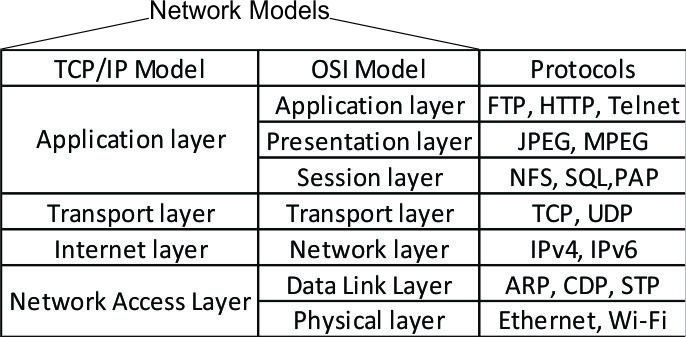
\includegraphics[height=4cm]{TVY-POS/ISO-OSI-TCP-IP/tcpip.jpg}
\end{multicols}
V koncových uzlech jsou implementovány všechny vrstvy pro kontrolu dat, v přechodových uzlech je implementována pouze síťová vrstva a vrstva síťového rozhraní.
Komunikace probíhá mezi sousedními vrstvami nebo mezi stejnolehlými vrstvami.
Pro komunikaci se používá buďto TCP, nebo UDP.
\subsection{IP}
Univerzální přenosový protokol k nespolehlivému, nespojovanému přenosu dat mezi zdrojovým počítačem a příjemcem.
Každé zařízení dostává nějakou indentifikaci v podobě IP adresy.
Přenášená data se nazývají IP datagramy neboli IP pakety, každý paket obsahuje hlavičku, ve které nese metadata a vlastní přenášená data.
Dnes se používají protokoly IPv4 a IPv6.
Cesta není předem vytyčena a optimální cestu nachází každý uzel, přes který daný paket jde.
Zpráva rozdělená na několik paketů nemusí dorazit ve stejném pořadí, jako byla poslána.
Každý poškozený paket síťová vrstva zahodí.
Požaduje-li aplikace spolehlivý přenos dat, jsou k dispozici protokoly vyšších vrstev.
Při přenosu velkých dat se mohou data fragmentovat.
Fragmentují se na vysílající stanici a defragmentují na přijímací.
\subsection{IEEE}
Jedná se o mezinárodní institum zabývající se výrobou standartů v oblasti internetového průmyslu.
Jejich protkoly se používají pro spoustu řešení v této problemice.
Od protokolu 802.1q pro trunk komunikaci ve VLAN až po 802.11 pro specikiaci WI-FI technologie.

\section{Polovodičové paměti}
\label{sec:polpameti}
Paměť je médium, které umožňuje uchovávat informace.
Základní paměťová buňka uchovává jeden bit informace - buďto logickou 0 nebo logickou 1.
Osm takových buňek tvoří jeden bajt.
Paměťové prvky jsou spojeny řádkovými a sloupcovými vodiči, pomocí kterých je možné je elektronicky ovládat.\\ \\
Parametry pamětí: \\
\begin{tabularx}{\linewidth}{l|l|l}
  \textbf{Parametr}  & \textbf{Jednotka} & \textbf{Popis}                                                        \\
  \hline
  Kapacita           & Bajt              & Množství informací, které lze do paměti uložit                        \\
  \hline
  Přístupová doba    & Sekunda           & Doba, od zadání požadavku, než paměť zpřístupní požadovanou informaci \\
  \hline
  Přenosová rychlost & Bajt za skundu    & Množství dat, které lze přečíst/zapsat za sekundu                     \\
  \hline
  Šířka toku dat     & Bit               & Počet bitů, které se po sběrnici přenášejí současně                   \\
  \hline
  Cena za bit        & Koruna za bit     & Cena za jeden bit paměti.                                             \\
  \hline
  Spolehlibost       & Sekunda           & Střední doba mezi 2 poruchami                                         \\
\end{tabularx}
\subsection{Dělení pamětí}
\subsubsection{Podle určení}
\begin{description}
  \item[Registry] - Paměti na čipu procesoru pro krátkodobé uložení dat.
    Malá kapacita, ale velmi vysoká rychlost.
  \item[Vnitřní] - Paměti na základové desce, slouží jako paměť programů a jejich data.
  \item[Vnější] - Vyměnná média a disky.
    Data jsou zaznamenávána magneticky, elektricky nebo opticky.
\end{description}
\subsubsection{Podle principu činnosti}
\begin{description}
  \item[Statická] - Pamět uchovávají informaci po dobu přívodu el. napětí.
    Mají nízkou přístupovou rychlost, ale jsou složité a drahé (Cache).
  \item[Dynamická] - Ztrácí informaci i když jsou připojené k el. napětí, proto je nutné je periodicky oživovat.
    Tvoří je transistor a kondenzátor. Mají vyšší přístupovou dobu, ale nižší náklady (Operační paměť).
\end{description}
\begin{multicols}{2}\centering
  SRAM
  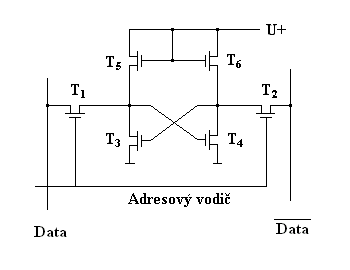
\includegraphics[width=\linewidth]{TVY-POS/Polovodicove-pameti/SRAM.png}
  \columnbreak\centering

  DRAM
  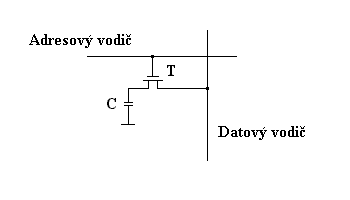
\includegraphics[width=\linewidth]{TVY-POS/Polovodicove-pameti/DRAM.png}
\end{multicols}
\subsubsection{Podle destruktivnosti při čtení}
\begin{description}
  \item[Destruktivní] - Paměť po přečtení informace ztrácí tuto informaci a je nutné ji znovu zapsat.
  \item[Nedestruktivní] - Uchovává informaci i po jejím přečtení.
\end{description}
\subsubsection{Podle energetické závilosti}
\begin{description}
  \item[Volatilní] - Paměť \textbf{NE}uchovává informaci po odpojení od el. napětí.
  \item[Non volatilní] - Paměť uchovává informaci i po odpojení od el. napětí.
\end{description}
\subsubsection{Podle přístupu}
\begin{description}
  \item[Sekvenční] - Před zpřístupněním informace je nutné přečíst všechny předcházející informace
  \item[Přímý] - Je možné přečíst přímo požadovanou informaci za pomocí její adresy
\end{description}
\subsubsection{Podle možnosti zápisu a čtení dat}
\begin{description}
  \item[ROM] - Data jsou zapsána při výrobě paměti. Realizováno vodičem nebo transistorem.
  \item[RWM] - Umožňují minimálně jeden zápis. Lze relizovat pomocí:
    \begin{itemize}
      \item PROM - Přepolování drátků. Pouze jeden zápis.
      \item EPROM - Elektronický zápis a mazání pomocí UV. Možnost více zápisů.
      \item EEPROM - Elektronický zápis i čtení. Možnost více zápisů.
    \end{itemize}
\end{description}
\subsubsection{Podle technolgie}
\begin{description}
  \item[Bipolární] - Buňky jsou tvořené bipolárními tranzistory
  \item[Unipolární] - Buňky josu tvoření tranzistory MOS
\end{description}
\subsection{R/W Cyklus buňky}
Vždy je udána adresa paměťového místa, se kterým se pracuje.
Adresa je přivedena na vstup dekoréru, která podle adresy nastaví adresový vodič na logickou 1.
Jestliže buňkou na tomto adresném vodiči projde logická 1 na datový vodič, tak je hodnota bitu logická 1.
V případě že buňkou logická 1 neprojde, pak je hodnota bitu 0.
U zápisu je dána opět adresa místa, kam se bude zapisovat, poté se nastaví hodnoty jednotlivých bitů a zapíšou se.

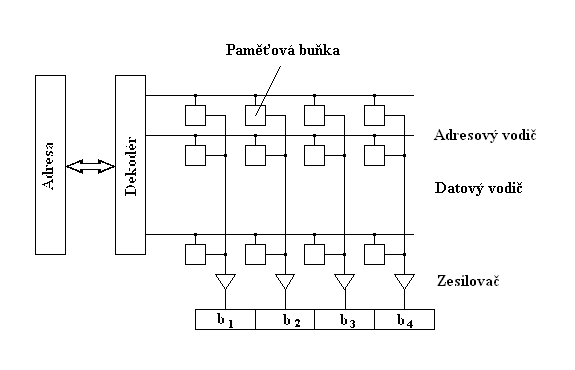
\includegraphics[width=\linewidth]{TVY-POS/Polovodicove-pameti/memorystructure.png}
\section{Fyzická vrstva}
\label{sec:fyzicka-vrstva}
Jedná se o nijižší vrstvu ISO-OSI modelu.
Zajišťuje fyzické spojení obou stran.
Patří do ní kabeláž, HW, konektory, vysílače, příjimače aj.
Definuje elektrické, mechanické, optické a elektromagentické vlny a jejich vlastnosti.
Informace přenáší ve formě bitů - kabely, vlny a světlo neznají ale bity - je nutné definovat jaký stav znamená log. 1 a co log. 0.
Komunikace probíhá oběžníkovým způsobem a je řízena Linkovou vrstvou.
\subsection{Zařízení pracující na fyzické vrstvě}
\begin{description}
  \item[Zesilovač]- Zesiluje signál i se šumem, je jednodušší, levnější a rychlejší než opakovač
  \item[Opakovač]- Regeneruje signál (Opraví, zesílí a načasuje), elektricky odděluje segmenty
  \item[HUB (Rozbočovač)]- Navyšuje konektivitu, regeneruje signál, rozvětvuje signál do více výstupů
\end{description}
\subsection{Přenosová média}
Mezi vlastnosti přenosových médií patří:\\
\begin{tabularx}{\linewidth}{l|l|l}
  \textbf{Parametr}    & \textbf{Jednotka} & \textbf{Popis}                                      \\
  Přenosová rychlost   & Bajt za sekundu   & Množství dat, které lze přenést za sekundu          \\
  \hline
  Útlum signálu        & dB na vzdálenost  & Zeslabení signálu po průchodu určitou délkou vodiče \\
  \hline
  Odolnost vůči rušení & ---               & Zejména proti elektromagickému rušení               \\
  \hline
  Zkreslení signálu    & ---               & Jaká změna nastala na signálu po průchodu médiem    \\
  \hline
  Fyzická odolnost     & ---               & Odolnost proti ohybu, tahu, mechická pevnost        \\
\end{tabularx}
\subsubsection{Kroucená dvojlinka}
Pravidelně zkroucený pár vodičů, většinou měděných.
V dnešní době se používá několik takových navzájem zkroucených párů.
Zkroucením se minimalizuje vyzařování elektromagentických vln a minimalizují se přeslechy.
Dnes používané hojně jako Patch kabely (Ethernet).
\subsubsection{Koaxilní kabel}
Kabel s vnitřním vodičem a druhým válcovým vnějším vodičem.
Navzájem jsou vodiče odděleny dielektrikem.
Průmery kabelů jsou od milimetrů po desítky centimetrů.
Používají se pro televize.
\subsubsection{Optické kabely}
Přenášejí data pomocí světelného paprsku.
Jsou mnohem dražší a komplikovanější než metalické vodiče.
Zdrojem světla bývají LED či laserové diody.
Pro přenos ve využívá \textbf{totálního odrazu} (Fyzikální zákon, který umožňuje odrazit veškeré světlo pomocí přechodu světla z opticky hustšího prostředí do opticky řidšího)
Dělí se na:
\begin{description}
  \item[Jednovidová] - Přenáší pouze jeden světelný paprsek
  \item[Mnohovidová] - Přenáší více světelných paprsků
\end{description}
\subsubsection{Rádiové spoje}
Jedná se o přenosy elektromagentických vln v určitém rozsahu elektromagentického spektra.
Hlavní výhodou tohoto spoje je absence kabelů, tudíž bezdrátová komunikace.
Nevýhodou je možnost oblivnění přenosu pomocí vlivů, které by u drátové nebyly problém.
Pro rádiové spoje se využívá různých frekvečních délek například 87.6 Mhz (Rádio Impuls) a 5 Ghz (Wi-Fi).
Mezi další technologie hojně využívající rádiové spoje patří: Bluetooth, Mobilní signál, GPS aj.
\subsection{Druhy možností šíření signálu}
\subsubsection{Sériové a paralelní přenos}
\begin{description}
  \item[Sériové spoje]- Bity jdou za sebou postupně jedním vodičem. Bajty jsou tvořeny posloupností bitů.
  \item[Paralelní spoje]- Několik bitů se posílá současně pomocí více vodičů. Obvykle se přenáší celý bajt.
\end{description}
\subsubsection{Synchronní a asynchronní přenos}
\begin{description}
  \item[Synchronní spoje]- Přenos dat probíhá společně se signálem CLK, který generuje pouze jedna strana.
  \item[Asynchronní spoje]- Každá strana si CLK generuje sama. Komunikace začíná pomocí start a stop bitu.
\end{description}
\subsubsection{Symetričnost singálu}
\begin{description}
  \item[Symetrický signál]- Přenos probíhá dvou vodičím v opačné polaritě. Výstupní signál je rozdíl přenosů.
  \item[Asymetrický signál]- Přenos probíhá po jednom vodiči. Náchylné na poruchy, nižší spolehlivita.
\end{description}
\section{Síťová vrstva}
Zajišťuje přenos dat mezi vzdálenými počítači (WAN).
Klíčovým prvkem v této komunikaci je směrovač (router).
Každý takový směrovač má svoji jednoznačnou identifikaci v rámci WAN (IP Adresu).
Přenáší se IP datagramy neboli pakety. Nezajímá se o protokoly linkové a fyzické vrstvy.\\
Funkce síťové vrstvy:
\begin{itemize}
  \item Hledání cesty pro pakety mezi libovolnými dvěma uzly v síti
  \item Nestará o spolehlivost, ale o co nejrychlejší přenos dat
  \item Zajistění postupného přenosu paketů přes mezilehlé uzly v cestě
  \item Přenosový protokol IP se snaží zakrývat rozdíly v technologiích nižší vrstvy
\end{itemize}
Cesta paketu:
\begin{enumerate}
  \item Zabalení přenášeného paketu do rámce
  \item Prostřednictvím vrstvy síťového rozhraní předání rámce přímému sousedovi
  \item V sousedním uzlu přijmutí a rozbalení rámce vrstvou síťového rozhraní
  \item Předání získaného paketu své síťové vrstvě, která najde nejvhodnější cestu k cíli
  \item Prostřednictvím vrstvy síťového rozhraní zaslání rámce k dalšímu uzlu
\end{enumerate}
\subsection{Směrování}
Technika k vnitřnímu rozčlenění rozsáhlých sítí LAN i MAN.\\
Běžně se používá jako proces šíření globální síťové komunikace v Internetu.\\
Účely směrování:
\begin{itemize}
  \item Usměrnění komunikace
  \item Optimalizace zátěže sítě
  \item Implementace bezpečnosti
  \item Zvýšení spolehlivosti na síťové vrstvě
\end{itemize}
\begin{description}
  \item[Statické]je nastaveno pevně administrativně - DHCP
  \item[Dynamické]je pravidelně aktuailzováno speciálními protokoly - Mnoho
\end{description}
\subsection{IP Adresace}
Každá síťová stanice musí mít pevně stanovenou identifikaci - IP adresu.
Ta je buďto napevno přidělena nebo dynamicky přidělována.
V současné době se využívá IPv4 adresa o velikosti 32bitů.
Tato IP adresa má v sobě zahrnuté jak číslo sítě, tak číslo stanice.
Tvar adresy je \[XXX.XXX.XXX.XXX\]
V každé síti musí být jedinečný router, který síť propojuje pomocí směrování. IP adresa hostitele a routeru musí být odlišná.\\
Jiné protkoly dostupné pro síťovou vrstvu: ICMP - Internet Control Message Protocol (Řešení problémů IP, ping\dots), IGMP, ARP, RARP.

\section{Motherboard}
\label{sec:motherboard}
Deska plošných spojů, která elektricky a fyzicky propojuje jednotlivé komponenty počítače.
Funkce základní desky:
\begin{enumerate}
  \item Napájet komponenty
  \item Mechanicky udržet komponenty u sebe
  \item Umožnit rychlý a spolehlivý přenos dat z jedné periférie do druhé
\end{enumerate}
Možnosti zapojení komponent k základní desce:
\begin{itemize}
  \item Interně - Porty a vstupy uvnitř case na základní desce
  \item Externě - Porty a vstupny z vnější strany case, taktéž na zákldní desce
\end{itemize}
Základní desky nejsou jenom v počítačích, ale i noteboocích, mobilech aj.\\
Velikosti základních desek: E-ATX, ATX, mATX, ITX\dots
\subsection{Blokové schéma a jednotlivé komponenty}
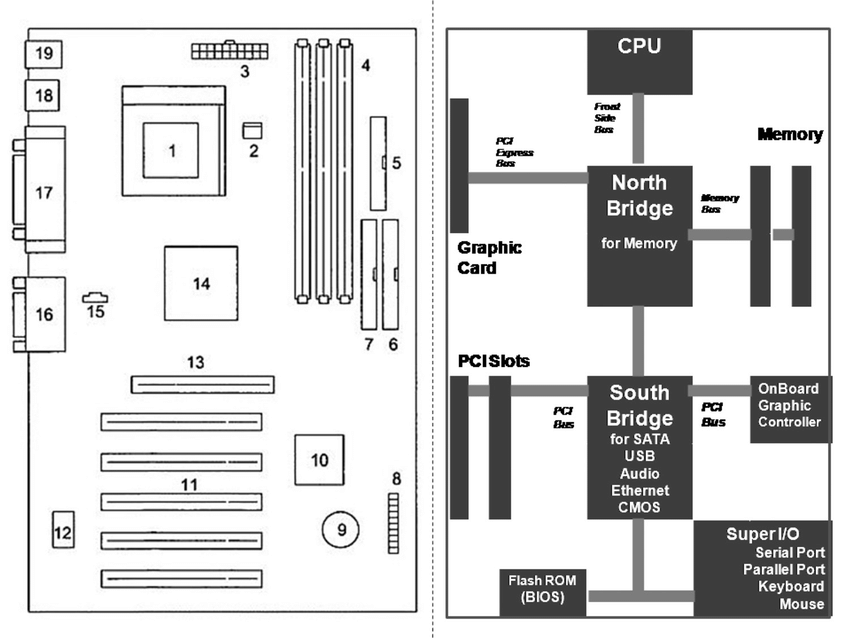
\includegraphics[width=1\linewidth,height=0.58\linewidth]{TVY-POS/Motherboard/MB.png}
Popis fyzického schéma:\\
\begin{enumerate}
  \item[1)] Patice CPU - Rozdíl mezi AMD (AM4, AM3) a Intel (12th gen LGA1700)
  \item[2)] CPU FAN Header - Pro chlazení CPU, jiné usazení chladiče pro AMD a Intel
  \item[3)] ATX napájení - Napájení základní desky a jejich komponent
  \item[4)] DDR sloty - Rozdíl mezi DDR3, DDR4, DDR5 (Umístění mezery)
  \item[8)] Porty pro case - HD Audio, USB, PWR, Reset, HDDLED, PWRLED
  \item[9)] RTC - Hodiny reálného času, baterie + kondenzátor, 32.768 kHz, 1.7 sekundy chyba denně
  \item[10)] Southbridge - Propojení NB a Serial \& Paralel port, PS2 klávesnice, myš
  \item[11)] PCI - Univerzální rozšiřující sloty. x4, x8, x16
  \item[12)] BIOS - Flash pamět se zaváděcím systémem
  \item[13)] PCI-E - Vysokorychlostní rožšiřující slot, v dnešní době hlavně pro grafické karty.
  \item[14)] Northbridge - Rozhraní pro propojení CPU s opereační pamětí a PCI-E
  \item[15)] FAN Header - Napájení a ovládání
  \item[] CPU napájení - Chybí na obrázku
\end{enumerate}

\section{Laserové a LED tiskárny}
\label{sec:tiskarny}
Tiskárna je výstupní zařízení, které slouží k přenosu dat uložených v elekronické podobě na papír nebo jiné médium.

Tiskárnu připojujeme k počítači (USB, Bluetooth, Síť\dots), ale může fungovat i samostatně a nebo být přímo součástí multifunčních zařízení jako pokladna nebo lékařské přístroje.
Tiskárny se ovládají pomocí jazyku PCL nebo Postskript.

Kvalitu tisku určuje rozlišení v podobě počtu bodů na palec (DPI) a počtů pixelů na palec (PPI).
Tiskárny nedokáží vytisknout jeden pixel libovolné barvy a tak většinou musí namíchat barvu z několika bodů na jeden pixel obrazu.
Bod proto musí být menší jak pixel.
Výjimku tvoří sublimační tiskárna, která barvy kondenzuje v jednom místě.
\subsection{Laserové tiskárny}
Pracuje na xerografickém principu.
Vyznačují se tichým chodem, nízkými provozními náklady a vysokou rychostí.
Na druhou stanu bývají dražší a potřebují čas na zahřátí.
Není vhodná pro fotografie.
Postup tisku:
\begin{enumerate}
  \item Povrch válce se v celé šírce nabije z korony
  \item Válec se osvítí laserem na bodech, které se mají vytisknout, čímž na daném místo sníží odpor polovodiče a náboj se poté z povrchu vybije do středu válce.
  \item Toner, vlivem otáčení nabit stejnou polaritou jako povrch válce, přilne k válci pouze na místech, kde byl odstraněn náboj.
  \item V ostatních místěch je toner od válce odpuzován, protože má stejnou polaritou
  \item Toner se s neutrálním nábojem přenese na papír, který je nabit na opačnou hodnotu než povrch válce
  \item Toner je pomocí teploty $\pm 180\degree C$ a tlaku roztaven a zapečen do papíru
  \item Z papíru je sejmut náboj a papír se uloží do výstupního zásobníku
  \item Mechanický stěrač setře zbytky toneru z válce
  \item Žárovka odstraní náboj z předchozího tisku
\end{enumerate}
\input{TVY-POS/Laserove-a-LED-tiskarny/laser-printer.pdf_tex}
\subsection{LED tiskárny (XEROX)}
Funguje podobně jako laserová tiskárna.
Místo osvícení pomocí laseru se zde využívají dvě a více řad LED diod.
Tudíž se ozařuje celý papír naráz a odpadá nutnost mecahnické části rotace laseru.\\
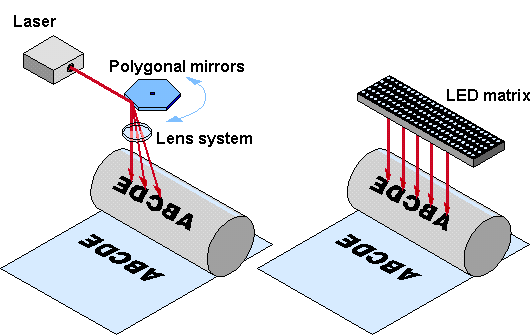
\includegraphics[width=1\linewidth]{TVY-POS/Laserove-a-LED-tiskarny/LEDandLaserPrinter.png}

\section{Vstupní zařízení}
\subsection{Klávesnice}
Klávesenice předává informace o stlačených klávesách operačnímu systému zpracované BIOSem.
Připojují se fyzicky pomocí USB a PS2 konektoru nebo bezdrátově pomocí Bluetooth či infračerveného záření.
Informace jsou ve SCAN kódu, kde se začíná klávesou ESC na čísle 1 a pokračuje se dál po řádcích.
Postup přenosu stisku:
\begin{enumerate}
  \item Mikroprocesor vestavěný do klávesnice nebo základové desky neustále monitoruje stav klávesnice
  \item Změna stavu způsobí vysílání kódu do základové desky klávesnice
  \item Stisk musí trvat aspoň 2 nebo 3 cykly, jinak se ignoruje
  \item Po uvolnění klávesy se kód klávesy zvýší o 128
  \item Číslo se uloží do paměti klávesnice a mikroprocesorem se zapíše na port
  \item Nastane přerušení a BIOS čte kód klávesy
  \item Po přečtení BIOS sdělí klávesnici pokyn o vymazání klávesy
  \item Při delším stisku se generuje signál stlačené klávesy
  \item BIOS dále testuje ještě 2 byty klávesnice na portu pro případné speciální funkce jako CTRL, ALT, aj.\\
        Tyto funkce se zapisují do bytů na adrese 0417H a 0418H
\end{enumerate}
\subsubsection{Mechanické klávesnice}
Potlačením tlačítka se mechanicky spojí vodiče. Pružinou se klávesa vratí zpátky.\\
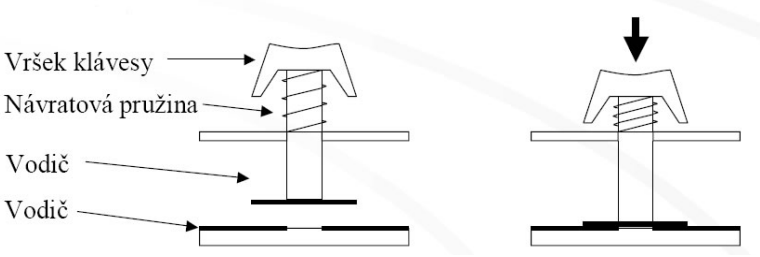
\includegraphics[width=1\linewidth]{TVY-POS/Vstupni-zarizeni/mechanickey.png}
\subsubsection{Membránové klávesnice}
Protlačením membrány dojde ke styku kontaků. Většinou pomocí mikrospínačů.\\
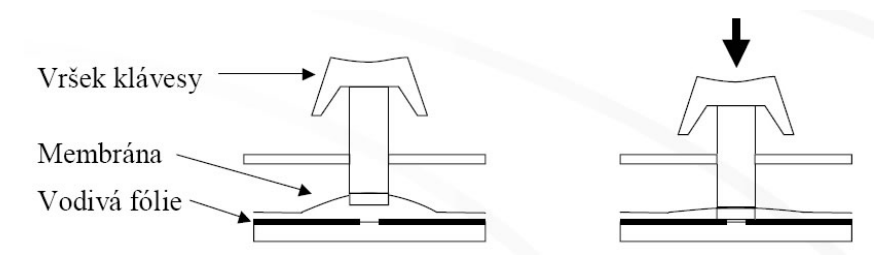
\includegraphics[width=1\linewidth]{TVY-POS/Vstupni-zarizeni/membranekey.png}
\subsubsection{Kapacitní klávesnice}
Přiblížení jádra k dorazu změní kapacitu kondnzátoru.
Není zde žádný dotek.
Jádrem je dielektrikum, které je pružinou oddalování.\\
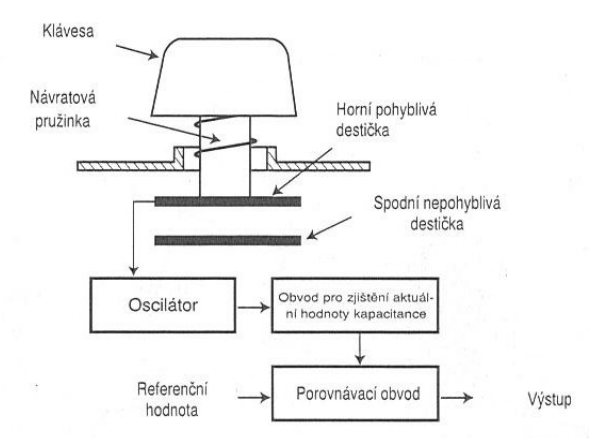
\includegraphics[width=1\linewidth]{TVY-POS/Vstupni-zarizeni/capacitorkey.png}
\subsubsection{Hallovy klávevy}
Klávesy mají uvnitř permanentní magnet.
Pod klávesou je Hallova sonda, která reguje za změnu magentického pole.
Při stisku klávesy se magnet přiblíží k Hallově sondě, která jako reakci vyšle elektrický signál.
Změnou magnetického pole pohybem klávesy se změní napětí na výstupu.
Takové klávesnice jsou velmi kvalitní, ale drahé.
\subsubsection{Dotykové klávesnice}
Dotyky se detekují pomocí změny kapacity kondenzátoru změnou dielektrika, který představuje prst.
Bez pohyblivých částí.
\subsection{Tablety}
Jsou to snímací podložky funkčně podobné grafickým stolům.
Využívají se ke kreslení vektorových obrazců.
Po podložce se pohybuje snímací zařízení, většinou myš se zaměřovačem nebo pero.
Myš místo kuličky obsahuje vysílací cívku, která vysílá impulsy čtené podložkou pomocí sítě snímačů.
Obsahuje lupu pro přenou polohu a tlačítka.
V peru bývá tlakový senzor pro určení tloušťky čáry.
\subsection{Světelná pera (Optická, Light Pen)}
Světelné pero snímá pozici pera na monitoru pomocí grafického adaptéru.
V peru je snímač světla, který identifikuje polohu pomocí bodu na monitoru.
Pracuje s informací, kdy se bod na monitoru obnoví, pomocí které určí, kde se pero nachází.
Monitor musí obraz vysílat řádek po řádku, bod po bodu.
\subsection{Dotykové obrazovky}
Existuje několik druhů dotykových obrazovek
\subsubsection{Rezistivní displeje}
Obrazovku tvoří pružná membrána.
Stiskem membrány spojíme elektrický proud.
Na základě velikosti jednotlivých proudů se vypočítá poloha displeje.
\subsubsection{Kapacitní dotykové dispeje}
Funguje na základě vodivosti lidského těla.
Dotykem prstu na displej se uzavře elektrický obvod a vytvoří se kapacita.
Řadič na základě velikosti kapacity určí polohu prstu.
\subsubsection{Dotykové displeje s IR}
Kolem displeje je rám vysílající IR paprsky.
Vsunutím předmětu se paprsek na daném místě přeruší.
\subsubsection{Displej s povrchovou akustickou vlnou (SAW)}
V rozích displeje jsou vysílače a přjímače 5Mhz sígnálu.
Přijímače vyhodnucují změnu šíření těchto vln a podle toho vyhodnutí polohu rušení.
Problematická je citlivost, jelikož malé znečištění je stále fatální.
\subsection{Myši}
Je to malé polohovací zařízení, která přenáší informace o svém pohybu do počítače.
Většinou se toto projeví jako pohyb kruzoru.
Mívá tlačíka a kolečko.
Připojovala se pomocí sériového RS-232 portu, poté se používal PS/2 a nyní USB.
Některé myši se dají pomocí redukce připojit do PS/2 či USB.
Existují i bezdrátové myši, u kterých se využívá buďto IR (IrDA) nebo rádiových vln (Např.: Bluetooth).
\subsubsection{Mechanická myš (Kuličková)}
Zespod myši je kulička, která se pohybem roztáčí.
Otáčení kuličky snímají dvě navzájem kolmé hřídele.
Hřídele při svém pohybu přenáší pohyb na otočnou clonu ve tvaru kruhu s okny.
Každé pootočení clony přeruší paprsek, což je přeneseno na elektrický impulz.
Rozpoznává se směr otáčení pomocí Grayova kódu.
Impulzy myši tvoří 2 a 2 bity, která se pak převádí na pohyb po X a Y na obrazovce.
\subsubsection{Optická myš}
Myš vysílá LED nebo laser, který se snímá fotodiodami nebo jiným optickým snímačem.
Pohyb myši se poté v reálném čase převádí do os X a Y.
Infračervené záření má vyšší přesnost a nižší spotřebu, ale ve skutečnosti na světle nezáleží.
Myš funguje lépe na strukturovaném povrchu, kde je možné snadno rozpoznat pohyb podkladu.
\end{document}
